%%%%%%%%%%%%%%%%%%%%%%%%%%%%%%%%%%%%%%%%%%%%%%%%%%%%%%%%%%%%%%%
\section{zkEVM Architecture}


\subsection{Registries}

In order to replicate the EVM opcodes, zkEVM introduces six state related generic registers named \A, \B, \C, \D and \E. However, since zkEVM operates over a finite field of almost 64 bits, each register is split into 8 limbs of 32 bits each: 
\begin{align*}
    &\A_0, \dots,  \A_7 \\
    &\B_0, \dots,  \B_7 \\
    &\C_0, \dots,  \C_7 \\
    &\D_0, \dots,  \D_7 \\
    &\E_0, \dots,  \E_7 \\
\end{align*}
with $\A_i, \B_i, \C_i, \D_i, \E_i \in \{0, \dots, 2^{32} - 1\}$. When storing a value in a register, the least significant bits are placed in the lowest limb, starting from the $0$-th one. That is, if we want to allocate a $32$ bits value in the \A-th register, we will fill only $\A_0$ with it. It we want to allocate a $64$ bits value, we will fill $\A_0$ and $\A_1$ and so on.  For example, if one want to store the value \texttt{0x12345678} in the \A register, the least significant byte \texttt{0x78} would be placed in $\A_0$ and the most significant byte \texttt{0x12} in $\A_3$. 

Apart from the generic registers related with the state of the zkEVM, there are additional registers in zkEVM that are used for various purposes. Here is a brief description of each of these registers:

\begin{itemize}
    
    \item \texttt{SR}: This is the status register and is used to indicate the current status of the processor. For example, it might indicate whether an arithmetic operation resulted in a carry or overflow, or whether an instruction encountered an error.
    
    \item \texttt{CTX}: This is the context register and is used to store the context of the current execution environment. For example, it might store information about the current smart contract being executed or the current transaction.
    
    \item \texttt{SP}: This is the stack pointer register and is used to point to the top of the stack. Every time a number is pushed onto the stack or removed from it, it is either increased or decreased. 
    
    \item \texttt{PC}: This is the EVM program counter register. The Program Counter (\texttt{PC}) encodes which instruction, stored in the code, should be next read by the EVM.  The program counter is usually incremented by one byte, to point to the following instruction, with some exceptions. For instance, the \texttt{PUSHx} instruction forces the \texttt{PC} to skip their parameter because it is longer than a single byte. The \texttt{JUMP} instruction modifies the program counter to a location determined by the top of the stack rather than increasing the \texttt{PC}'s value. 
    
    \item \texttt{GAS}: This is the gas register and is used to store the amount of gas remaining for the current transaction. Gas refers to the unit that measures the amount of computational effort required to execute specific operations on the Ethereum network.
    
    \item \texttt{RR}: This is the return register and is used to store the address to return to after a function call or jump.
    
    \item \texttt{zkPC}: This is the zkEVM program counter register. Similarly as explained in the \texttt{PC} register, it encodes which instruction of the zkEVM is being executed. This register will be crucial in order to ensure that the program that is being executed matches the program that wants to be proved. 
    
    \item \texttt{STEP}: This is the step register and is used to store the number of instructions executed so far in the current transaction.
    
    \item \texttt{MAXMEM}: This is the maximum memory register and is used to store the maximum amount of memory that can be allocated for the current transaction.
    
    \item \texttt{HASHPOS}: This is the hash position register and will contain the index of the next position of the bytes array of the input of the hash that we will start to fill. More information on that can be found in the hash-related instructions section. 
    
    \item \texttt{ROTL\_C}: This is the \C-rotate left (read-only) register and is used to flag a left rotation of the \C register by $4$ bytes. This has the effect of moving the $4$ most significant bytes of the \C register to the $4$ least significant bytes, and moving the $28$ least significant bytes to the $28$ most significant bytes. Later on, this rotated \C register can be assigned elsewhere. For example:
    
    \begin{zkasm}
        ROT_C + 2 => A
    \end{zkasm}
    increases by $2$ units the rotated value of \C and assigns it into the register \A.
    
    \item \texttt{RCX}: This is the repeat count register \texttt{RCX}, which is used in the repeat instruction. The repeat instruction allows for a certain instruction to be executed multiple times, based on the value stored in the \texttt{RCX} register. The \texttt{RCX} register is decremented by one each time the instruction is executed, until it reaches zero. The use of the \texttt{RCX} register in the repeat instruction allows for efficient execution of repetitive tasks, as it avoids the need for explicit loops in the code.
    
\end{itemize}

Each of these registers serves a specific purpose in the operation of zkEVM and is used by the various instructions and operations defined in the zkEVM specification.








\subsection{Binary} \label{sec:binary-sm}

The zkEVM contains a specific state machine in order to perform several $256$-bits operations. Each one of them are programmed in order to operate between the registers \A and \B. The implemented operations are the following:

\begin{itemize}
    
    \item \ADD ($+$). This operation adds two 256-bit strings. Invoked using \texttt{:ADD} instruction. 
    
    \item \SUB ($-$). This operation subtracts two 256-bit strings. Invoked using \texttt{:SUB} instruction. 
    
    \item \LT ($<$). This operation checks if a 256-bit string is smaller than another 256-bit string considering a codification of the binary strings without sign. Invoked using \texttt{:LT} instruction. 
    
    \item \SLT ($<$). This operation checks if a 256-bit string is smaller than another 256-bit string but considering a codification of the binary strings with sign (the codification used by the EVM is complement to two). Invoked using \texttt{:SLT} instruction. 
    
    \item \EQ ($=$). This operation checks if two 256-bit strings are equal. Invoked using \texttt{:EQ} instruction. 
    
    \item \AND ($\land$). This operation computes the bit-wise ``add" of the two strings. Invoked using \texttt{:AND} instruction. 
    
    \item \OR ($\lor$). This operation computes the bit-wise ``or" of the two strings. Invoked using \texttt{:OR} instruction. 
    
    \item \XOR ($\oplus$). This operation computes the bit-wise ``xor" of the two strings. Invoked using \texttt{:XOR} instruction. 
    
\end{itemize}

To understand how the \ADD, \SUB, \LT and \SLT operations work, we need to understand in first place how the EVM codes $256$-bit strings to signed and unsigned integers. Figure \ref{fig:3-bit-strings} shows these codifications for 3-bit strings but the idea can be easily extended to 256-bit strings.

\begin{figure}[h!]
    \centering
    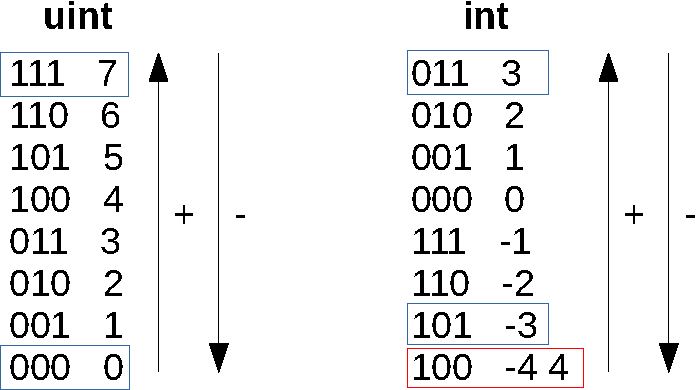
\includegraphics[width=0.55\textwidth]{../figures/integers_complement_two}
    \caption{Codifications of 3-bit strings for signed and unsigned integers as used by the EVM. \label{fig:3-bit-strings}}
\end{figure}


Adding two strings is performed bit by bit using the corresponding carry. For example, let's add the 3-bit strings $\texttt{0b001}$ and $\texttt{0b101}$:

\begin{itemize}
    
    \item We start with an initial $\texttt{carry}=0$ and adding the least significant bits: 
    
    $1+1+\texttt{carry}=1+1+0=0$ with the next carry being equal to $1$.
    \item Then, we add the next bits using the previous carry: 
    
    $0+0+\texttt{carry} = 0+0+1 = 1$ with the next carry being equal to $0$.
    \item Finally, we add the most significant bits: 
    
    $0+1+\texttt{carry}=0+1+0=1$ with the final carry being equal to $0$.
    \item As a result: $\texttt{0b001} + \texttt{0b101} = \texttt{0b110}$ with $\texttt{carry}=0$.
    
\end{itemize}

The sum $\texttt{0b001} + \texttt{0b101} = \texttt{0b110}$, for unsigned integers is $1+5=6$, while for signed integers encoded with complement to two this sum is $1+(-3) =(-2)$. In other words, we can do the same binary sum for both signed integers and for unsigned integers.

The operations \LT and \SLT are different however. When comparing unsigned integers (LT), the natural order for comparisons is applied, e.g. 110 (6) > 010 (2). When comparing signed integers (\SLT), we must take into account the most significant bit that acts as the sign. If the most significant bit of the two strings being compared is the same, the the natural order applies, e.g. 110 (-2) > 101 (-3). However, if the strings being compared have a different most significant bit, then the order must be flipped (bigger numbers start with 0), e.g. 001 (1) > 110 (-2). Finally, notice that with unsigned integers, there is a caveat since 4 and -4 have the same codification.

On the other hand, the \AND, \OR and \XOR operations are bit-wise operations, that is to say, the operation is done bit by bit. As a result, there are not any carries to be considered when operating a pair of bits. As we will see, this is going to make the checks easier to implement for bit-wise operations. Table \ref{tab:truth-tables} depicts the truth tables of \AND, \OR and \XOR operators, respectively.

\begin{figure}[h!]
    \[
    \begin{array}{|c|c|c|}
        \hline
        A 	&B 		&A \land B 	\\
        \hline
        0 	&0 		&0 				\\
        0 	&1 		&0				\\
        1 	&0 		&0 				\\
        1 	&1 		&1 				\\
        \hline
    \end{array}
    \hspace{0.5cm}
    \begin{array}{|c|c|c|}
        \hline
        A 	&B 		&A \lor B 	\\
        \hline
        0 	&0 		&0 				\\
        0 	&1 		&1				\\
        1 	&0 		&1 				\\
        1 	&1 		&1 				\\
        \hline
    \end{array}
    \hspace{0.5cm}
    \begin{array}{|c|c|c|}
        \hline
        A 	&B 		&A \oplus B 	\\
        \hline
        0 	&0 		&0 				\\
        0 	&1 		&1				\\
        1 	&0 		&1 				\\
        1 	&1 		&0 				\\
        \hline
    \end{array}
    \]
    \caption{Truth Tables of bit-wise operations}
    \label{tab:truth-tables}
\end{figure}

Notice that we do not consider the \textbf{NOT} operation. This is because the \textbf{NOT} operation can be easily implemented with the \XOR operation just by taking the 256-bit string and doing an \XOR with \texttt{0xff...ff}.



%TODO for Marc
\subsection{Arithmetic} \label{sec:arith-sm}


The Arithmetic State Machine (SM) is one of the six secondary state machines receiving instructions from the \textbf{Main SM} Executor. The main purpose of the Arithmetic State Machine is carry out elliptic curve arithmetic operations, such as Point Addition and Point Doubling as well as $256$-bits modular operations. The selected curve $E$ is the one with equation $y^2 = x^3 + 7$ over the field $\FF_p$ with:
\[
p = 2^{256} - 2^{32} - 2^9 - 2^8 - 2^7 - 2^6 - 2^4 - 1.
\] 

More specifically, thee Arithmetic SM is responsible for the execution of the following operations:

\begin{itemize}
    
    \item \textbf{Field Arithmetic}:  Here, $y_2$ and $y_3$ are the result of performing field arithmetic over $x_1,y_1$ and $x_2$. That is:
    
    \begin{equation}
        x_1 \cdot y_1 + x_2 = y_2 \cdot 2^{256} + y_3. \label{eq:field-arith}
    \end{equation}
    
    Note that if $y_1$ is set to $1$ then Eq. \eqref{eq:field-arith} represents field addition, and similarly if $x_2$ is set to $0$ then Eq. \eqref{eq:field-arith} represents field multiplication.
    
    \item \textbf{Elliptic Curve Addition}: Given two points $P = (x_1,y_1), Q = (x_2,y_2)$ from $E$ with $x_1 \neq x_2$, the point $P+Q = (x_3,y_3)$ is computed as follows:
    
    \begin{align*}
        x_3 &= s^2 - x_1 - x_2, \\
        y_3 &= s (x_1 - x_3) - y_1.
    \end{align*}
    
    where:
    \[
    s = \frac{y_2 - y_1}{x_2 - x_1}
    \]
    
    \item \textbf{Elliptic Curve Doubling}: Given a point $P = (x_1,y_1)$ from $E$ such that $P \neq \mathcal{O}$, the point $P+P = 2P = (x_3,y_3)$ is computed as follows:
    \begin{align*}
        x_3 &= s^2 - 2x_1, \\
        y_3 &= s (x_1 - x_3) - y_1.
    \end{align*}
    where:
    \[
    s = \frac{3x_1^2}{2y_1}.
    \]
    
\end{itemize}

Motivated by the implemented operations, the Arithmetic SM is composed of $6$ registers $x_1,y_1,x_2,y_2,x_3,y_3$. Each of these registers is decomposed in $16$ sub-registers of $16$-bit ($2$ byte) capacity, making a total of $256$ bits per register. We also need to provide $s$ and $q_0,q_1,q_2$, which are also elements of (the finite field) $256$ bits. 

The Arithmetic State Machine, combined with the Binary State Machine is used to implement opcodes like \textbf{signed and unsigned integer division}, \textbf{signed and unsigned module reducing}, \textbf{modular operations} or \textbf{exponentiation}. 







\subsection{Keccak-Related State Machines}


The KECCAK State Machine is in charge of validating the correct computation of EVM's KECCAK-256 hash. Unlike POSEIDON, due to its bit-wise nature, it is very inneficient in our set up and, therefore, it has been the focus for performing several optimizations. The strategy taken it is to use its circuit-like construction together with a PLONK-ish design in order to perform several KECCAK-f permutations at the same time. This State Machine is a complex one, because it has to deal with the Sponge Construction byte-wise and, later on, translate this execution bit-wise in order to compute all the KECCAK-f permutations in a parallel way. 

\subsubsection*{Sponge Construction}

The \textbf{sponge construction} is a simple iterated construction for building a function 
\[
F: \ZZ_2^* \to \ZZ_2^l
\] 
with variable-length input and arbitrary output length based on a fixed-length permutation
\[
f: \ZZ_2^b \to \ZZ_2^b
\] 
operating on a fixed number $b$ of bits. Here $b$ is called the \textbf{width}. The array of $b$ bits that $f$ keeps transforming is called the \textbf{state}. The state array is split in two chunks of $r$ and $c$ bits respectively. We call $r$ the \textbf{bitrate} (or rate) and $c$ the \textbf{capacity}. We will understand later on the motivation for this splitting. 

Let us describe how the sponge construction works:

\begin{enumerate}
    
    \item First of all, the input string is padded with a reversible \textbf{padding rule}, in order to achieve a length divisible by $r$. Subsequently, it is cut into blocks of $r$ bits. We also initialize the $b$ bits of the state to zero. 
    
    \item (\textit{Absorbing Phase}) In this phase, the $r$-bit input blocks are XORed into the first $r$ bits of the state, interleaved with applications of the function $f$. We proceed until processing all blocks of $r$-bits. Observe that the last $c$ bits corresponding to the capacity value does not absorb any input from the outside. 
    
    \item (\textit{Squeezing Phase}) In this phase, the first $r$ bits of the state are returned as output blocks, interleaved with applications of the function $f$. The number of output blocks is chosen at will by the user. Observe that the last $c$ bits corresponding to the capacity value are never output during this phase. Actually, if the output exceeds the specified length, we will just truncate it in order to fit. 
    
\end{enumerate}

We depict an schema of the sponge construction in Figure \ref{fig:sponge-construction}. 

\begin{figure}[H]
    \centering
    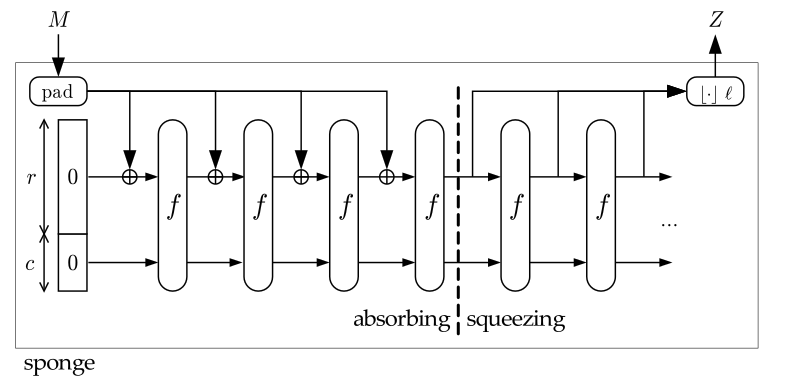
\includegraphics[width=0.6\columnwidth]{../figures/sponge-construction}
    \caption{Schema of Sponge Construction.}
    \label{fig:sponge-construction}
\end{figure}

The elements that completely describe a single instance of a sponge construction are: the fixed-length permutation $f$, the padding rule $\mathbf{pad}$ and the rate value $r$. 

\subsubsection*{EVM Hash Function Specification}

The EVM makes use of KECCAK-256 hash function, which is constructed using KECCAK$[512]$ sponge construction. Let us, therefore, define the KECCAK$[c]$ sponge construction. This sponge operates with a width of $1600$ bits and a rate of $1600 - c$. In the case of KECCAK$[512]$, the rate chunk is composed of $1088$ bits (or equivalently, $136$ bytes) and the capacity chunk has $512$ bits (or equivalently, $64$ bytes). The permutation used in KECCAK$[c]$ is KECCAK-$p[1600, 24]$ (See \cite{bertoni2013keccak}). The last ingredient we need to define in order to completely specify the hash function is the padding rule. In KECCAK$[c]$, the padding pad10*1 is used. If we define $j = (-m-2) \mod{r}$, where $m$ is the length of the input in bits, then the padding we have to append to the original input message is 
\[
P = 1 \mid\mid 0^j \mid\mid 1.
\]
Thus, given an input bit string $M$ and a output length $d$, KECCAK$[c](M, d)$ outputs a $d$ bit string following the previous sponge construction description. 

It should be noted that this construction does \textbf{not} follow the FIPS-202 based standard (a.k.a SHA-3). According to \cite{sha3standard}, NIST changed the SHA3 padding to
\[
\text{SHA3-256}(M) = \text{KECCAK}[512](M \mid\mid 01, 256).
\]
The difference is the additional $01$ bits appended to the original message, which were not present in the orignal KECCAK specification. 


\subsubsection*{zkEVM Keccak-related State Machines Pipeline}

Unlike the other state machines previously explained, rather than implementing the Keccak-256 hash function as a single state machine, the zkEVM does so in a framework of four state machines. They are as follows:

\vspace{3mm}
\begin{figure}[H]
    \centering
    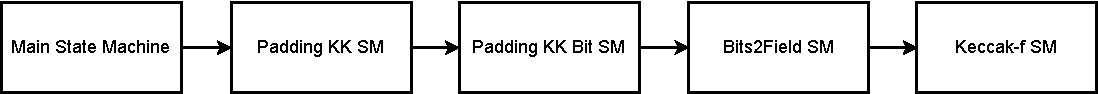
\includegraphics[width=0.9\columnwidth]{../figures/keccak-sm.drawio}
    \caption{Pipeline for Keccak-related State Machines.}
    \label{fig:keccak-sm}
\end{figure}

\begin{itemize}
    
    \item The \textbf{Padding KK} SM is used for padding purposes, as well as validation of hash-related computations pertaining to the \textbf{Main SM}'s queries. As depicted in the above figure, the \textbf{Padding KK SM} is \textbf{Main SM}'s gateway to the Keccak hashing state machines.
    
    \item The \textbf{Padding KK Bit} SM converts between two string formats, the bytes of the \textbf{Padding KK SM} to the bits of the \textbf{Keccak-f SM}, and vice-versa.
    
    \item The \textbf{Bits2Field SM} is used specifically for parallelizing \textbf{Keccak-f SM} implementation. It acts as a multiplexer between the \textbf{Padding KK Bit SM} and the \textbf{Keccak-f SM}. This state machine is called \textbf{Bits2Field} because it initially ensured the correct packing of bits from 4444 different blocks of the \textbf{Padding KK Bit SM} into a single field element.
    
    \item The \textbf{Keccak-F SM} computes string hashes at the request of the \textbf{Main SM}. Although the \textbf{Keccak-f SM} is a binary circuit, it operates on a 44bits-by-44bits basis rather than a bit-by-bit basis. This equates to running four 4444 hashing circuits in parallel.
    
\end{itemize}

\subsection{Poseidon-Related State Machines}

The \textbf{Poseidon State Machine} is a secondary state machine that receives instructions from the \textbf{Main State Machine} of the zkProver. It uses the Poseidon hash function to generate hash values in response to requests from the \textbf{Storage SM} (which we will see later on) and instructions from the \textbf{Main SM} Executor. Poseidon Actions are the directives that the \textbf{Poseidon SM} receives from one of the two SMs. It performs the Poseidon Actions as a secondary SM and also verifies that the output hash values were accurately calculated.


Poseidon (See \cite{poseidon}) is a hash function designed to minimize prover and verifier complexities when zero-knowledge proofs are generated and validated. The previously defined KECCAK-256 cryptographic hash require large circuits as they are not tailored to finite fields used in ZK proof systems (actually, KECCAK-256 works well in binary fields, and we will see later on that this fact introduces a lot of complexity in the constrain design). For this reason, zkEVM uses Poseidon hash as the main internal hash function. 

More concretely, we will now specify the specific instance of Poseidon that zkEVM uses. We will work over the field $\FF_p$ where $p = 2^{64} - 2^{32} + 1$. The state width of the Poseidon permutation is of $8$ field elements (observe that we are changing the paradigm, working with whole field elements instead of working bit-wise) meanwhile we will work with a capacity of $4$-field elements. 

The permutation used in Poseidon is a round function. A typical round function consists of three operations; an addition of a round-key $ARC(\cdot)$, a non-linear function $S$ (i.e., a substitution box or S-box), and a linear function $L$ which is often an affine transformation (in particular, an MDS matrix $M$). Some rounds are partial rounds because they use only one S-box instead of the full number of S-boxes, one for each element of the state. For security purposes against certain cryptanalytic attacks, outer rounds are full rounds, while the inner rounds are partial rounds. 

Denote the number of rounds by $R=R_F+R_P$ where $R_F$​ is the number of full rounds and $R_P$ is the number of partial rounds. Also, let $M(\cdot)$ denote the linear diffusion layer. Then, the figure blow depicts the Poseidon's permutation. 

\begin{figure}[H]
    \centering
    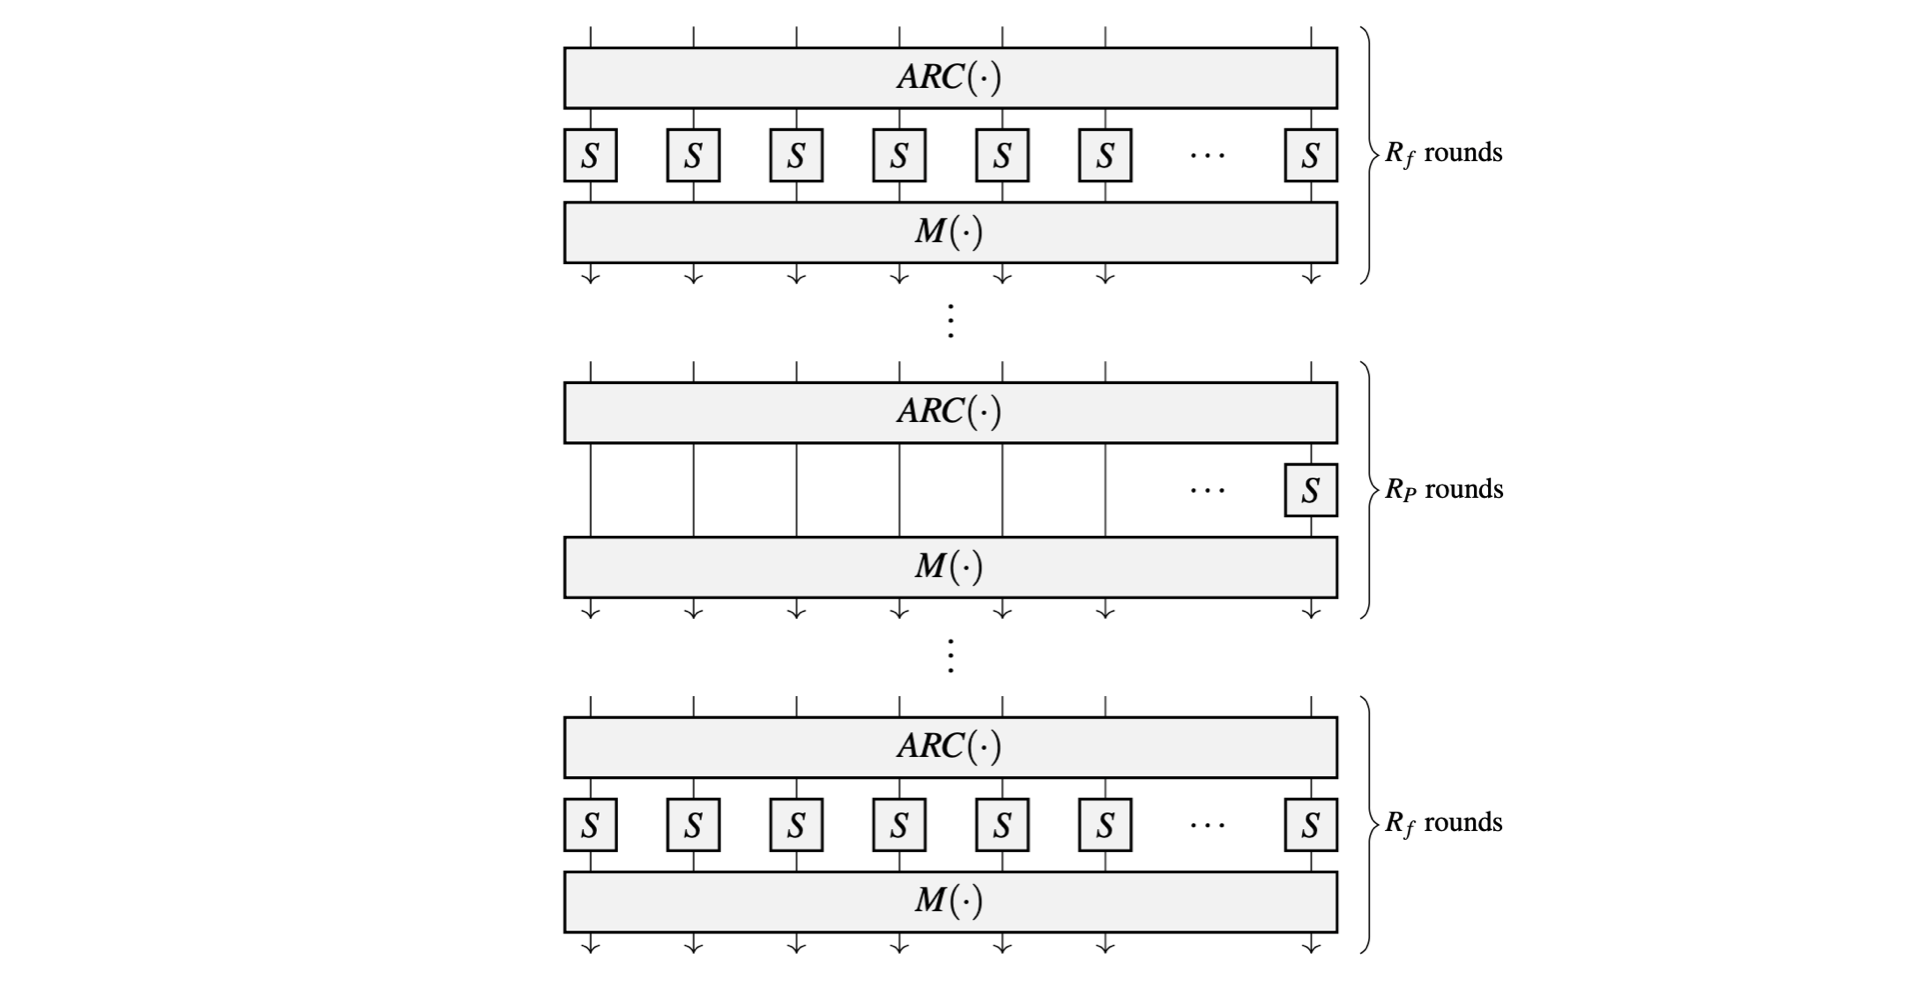
\includegraphics[width=\columnwidth]{../figures/poseidon-hades}
    \caption{HADES-based Poseidon's permutation.}
    \label{fig:poseidon-hades}
\end{figure}

The Poseidon S-box layer that we will use is the $7$-power S-Box, i.e.
\[
SB(x) = x^7,
\]
The Poseidon instance also requires to specify the number of full and partial rounds of the permutation. In our case, we will use 
\[
R_F = 8 \text{ (number of full rounds) }, \quad R_P = 22 \text{ (number of partial rounds)}
\]
Only one squeezing iteration will be effectuated, with an output of the first $4$ field elements of the state (which consists of approximately $256$-bits, but no more than that). The Round Constants and the MDS matrix are completely specified using the previous parameters. 



\subsection{Memory-Related State Machines}



\subsubsection*{Memory State Machine}


The memory of the EVM (Ethereum Virtual Machine) is a volatile read-write memory that
is used to store temporary data during the execution of transactions of smart contract functions. That is, data in memory is populated during transaction's execution but it does not persist between transactions. The memory is an array of $256$-bit ($32$ bytes) words that can be accessed through \textit{addresses at byte level}, that is to say, each byte in the memory has a different address. Memory has addresses of $32$ bits and initially, all memory locations are composed by bytes set to zero. Now, let's see the layout in memory of the following two words 0xc417...81a7 and 0x88d1...b723. Table \ref{tab:first-example} shows this layout.

\begin{figure}[h!]
    \[
    \begin{array}{|c|c|}
        \hline
        \mathbf{ADDRESS} &\mathbf{BYTE} \\ \hline
        \mathtt{0} &\mathtt{0xc4} \\
        \mathtt{1} &\mathtt{0x17} \\
        \mathtt{\vdots} &\mathtt{\vdots} \\
        \mathtt{30} &\mathtt{0x81} \\
        \mathtt{31} &\mathtt{0xa7} \\
        \mathtt{32} &\mathtt{0x88} \\
        \mathtt{33} &\mathtt{0xd1} \\
        \mathtt{\vdots} &\mathtt{\vdots} \\
        \mathtt{62} &\mathtt{0xb7} \\
        \mathtt{63} &\mathtt{0x23} \\
        \hline
    \end{array}
    \]
    \caption{Layout in memory of \texttt{0xc417...81a7} and \texttt{0x88d1...b723}.}
    \label{tab:first-example}
\end{figure}

Observe that each word has 32 bytes and that the words are stored in Big-Endian form, i.e. the most significant bytes are set in the lower addresses. The EVM provides three opcodes to interact with the memory area. We have an opcode to read and an opcode to write 32-byte words providing an offset:

\begin{itemize}
    
    \item \MLOAD: It receives an offset and returns the 32 bytes in memory starting at that offset.
    
    \item \MSTORE: It receives an offset and saves 32 bytes from the offset address of the memory.
    
\end{itemize}

Considering our previous memory contents, if we perform an \MLOAD with an offset of \texttt{1}, we would obtain the following word: \texttt{0x17...a788}. On the other hand, if we do an \MSTORE with an offset of \texttt{1} with the word \texttt{0x74f0...ce92}, we would modify the content of the memory as shown in Table \ref{tab:second-example}. 

\begin{figure}[h!]
    \[
    \begin{array}{|c|c|}
        \hline
        \mathbf{ADDRESS} &\mathbf{BYTE} \\ \hline
        \mathtt{0} &\mathtt{0xc4} \\
        \mathtt{1} &\mathtt{\textbf{0x74}} \\
        \mathtt{2} &\mathtt{\textbf{0xf0}} \\
        \mathtt{\ldots} &\mathtt{\ldots} \\
        \mathtt{31} &\mathtt{\textbf{0xce}} \\
        \mathtt{32} &\mathtt{\textbf{0x92}} \\
        \mathtt{33} &\mathtt{0xd1} \\
        \mathtt{\ldots} &\mathtt{\ldots} \\
        \mathtt{62} &\mathtt{0xb7} \\
        \mathtt{63} &\mathtt{0x23} \\
        \hline
    \end{array}
    \]
    \caption{Layout in memory after the introduction of \texttt{0x74f0...ce92}.}
    \label{tab:second-example}
\end{figure}

When the offset is not a multiple of 32 (or \texttt{0x20}), as in the previous example, we have to use bytes from two different words when doing \MLOAD or \MSTORE.

Finally, the EVM provides a write memory operation that just writes a byte:

\begin{itemize}
    
    \item \MSTOREE: It receives an offset and saves one byte on that address of the memory.
    
\end{itemize}

Notice that \MSTOREE always uses only one word.

The \textbf{Memory SM} is in charge of proving the memory operations in the execution trace. As mentioned, read and write operations use addresses at byte level in the EVM. However, doing the proofs byte by byte would consume many values in the trace of this state machine.

Instead, in this machine, we operate addressing words (32 bytes). For example, if we have the memory layout from Table \ref{tab:first-example}, then we would have the memory layout of Table \ref{tab:third-example} with addresses that point to 32-byte words.

\begin{figure}[h!]
    \renewcommand{\figurename}{Table}
    \[
    \begin{array}{|c|c|}
        \hline
        \textbf{ADDRESS} & \textbf{32-BYTE WORD} \\ \hline
        \mathtt{0} &\mathtt{0xc417...81a7} \\
        \mathtt{1} &\mathtt{0x88d1...b723} \\
        \hline
    \end{array}
    \]
    \caption{Layout in the memory state machine.}
    \label{tab:third-example}
\end{figure}

The \textbf{Memory SM} uses this latter layout, the 32-byte word access, to check reads and writes. However, as previously mentioned, the EVM can read and write with offsets at a byte level. As a result, we will need to check the relationship between byte access and 32-byte word access. For these checks, we have another state machine called \textbf{Memory Align SM} that is discussed below.


\subsubsection*{Memory Align State Machine} 



The \textbf{Memory SM} checks memory reads and writes using a 32-byte word access, while
the EVM can read and write 32-byte words with offsets at a byte level.
Table \ref{tab:byte:32byte:example} shows an example of possible byte-addressed and 32-byte-addressed memory layouts for the same content (three words).

\begin{figure}[h!]
    \renewcommand{\figurename}{Table}
    \[
    \begin{array}{|c|c|}
        \hline
        \mathbf{ADDRESS} &\mathbf{BYTE} \\ \hline
        \mathtt{0x00} &\mathtt{0xc4} \\
        \mathtt{0x01} &\mathtt{0x17} \\
        \mathtt{0x02} &\mathtt{0x4f} \\
        \mathtt{\ldots} &\mathtt{\ldots} \\
        \mathtt{0x1e} &\mathtt{0x81} \\
        \mathtt{0x1f} &\mathtt{0xa7} \\
        \hline
        \mathtt{0x20} &\mathtt{0x88} \\
        \mathtt{0x21} &\mathtt{0xd1} \\
        \mathtt{0x22} &\mathtt{0x1f} \\
        \mathtt{\ldots} &\mathtt{\ldots} \\
        \mathtt{0x3e} &\mathtt{0xb7} \\
        \mathtt{0x3f} &\mathtt{0x23} \\
        \hline
        \mathtt{0x40} &\mathtt{0x6e} \\
        \mathtt{0x41} &\mathtt{0x21} \\
        \mathtt{0x42} &\mathtt{0xff} \\
        \mathtt{\ldots} &\mathtt{\ldots} \\
        \mathtt{0x5e} &\mathtt{0x54} \\
        \mathtt{0x5f} &\mathtt{0xf9} \\
        \hline
    \end{array}
    \]
    \[
    \begin{array}{|c|c|}
        \hline
        \mathbf{ADDRESS} &\mathbf{32-BYTE~~WORD} \\ \hline
        \mathtt{0x00} &\mathtt{0xc4174f...81a7} \\
        \hline
        \mathtt{0x01} &\mathtt{0x88d11f...b723} \\
        \hline
        \mathtt{0x02} &\mathtt{0x6e21ff...54f9} \\
        \hline
    \end{array}
    \]
    \caption{Sample memory layouts for byte and 32-byte access.}
    \label{tab:byte:32byte:example}
\end{figure}

The relationship between the $32$-byte word addressable layout and the byte addressable layout is called ``memory alignment" and the \textbf{Memory Align SM} is the state machine that checks the correctness of this relationship. Notice that, in the general case, \MLOAD operation requires reading bytes of two different words. Considering that the content of the memory is the one shown at Table \ref{tab:byte:32byte:example}, since the EVM is addressed at a byte level, if we want to check a read from the EVM of a word starting at the address \texttt{0x22}, the value that we should obtain is the following:
\[
\val = \mathtt{0x1f \cdots b7236e21}.
\]
We denote the content of the words affected by an EVM memory read as $\mF$ and $\mS$.
In our example, these words are the following:
\[
\mF = \mathtt{0x} \mathtt{88d11f} \cdots \mathtt{b723},
\quad \mS =  \mathtt{0x} \mathtt{6e21ff} \cdots \mathtt{54f9}.
\]
We define a read block as the string concatenating the content of the words affected by the read: $\mF \mid \mS$.
Figure \ref{fig:mload-ex} shows the affected read words $\mF$ and $\mS$ that form the affected read block 
and the read value \val for a read from the EVM at address \texttt{0x22} in our example memory of Table \ref{tab:byte:32byte:example}.

\begin{figure}[h!]
    \centering
    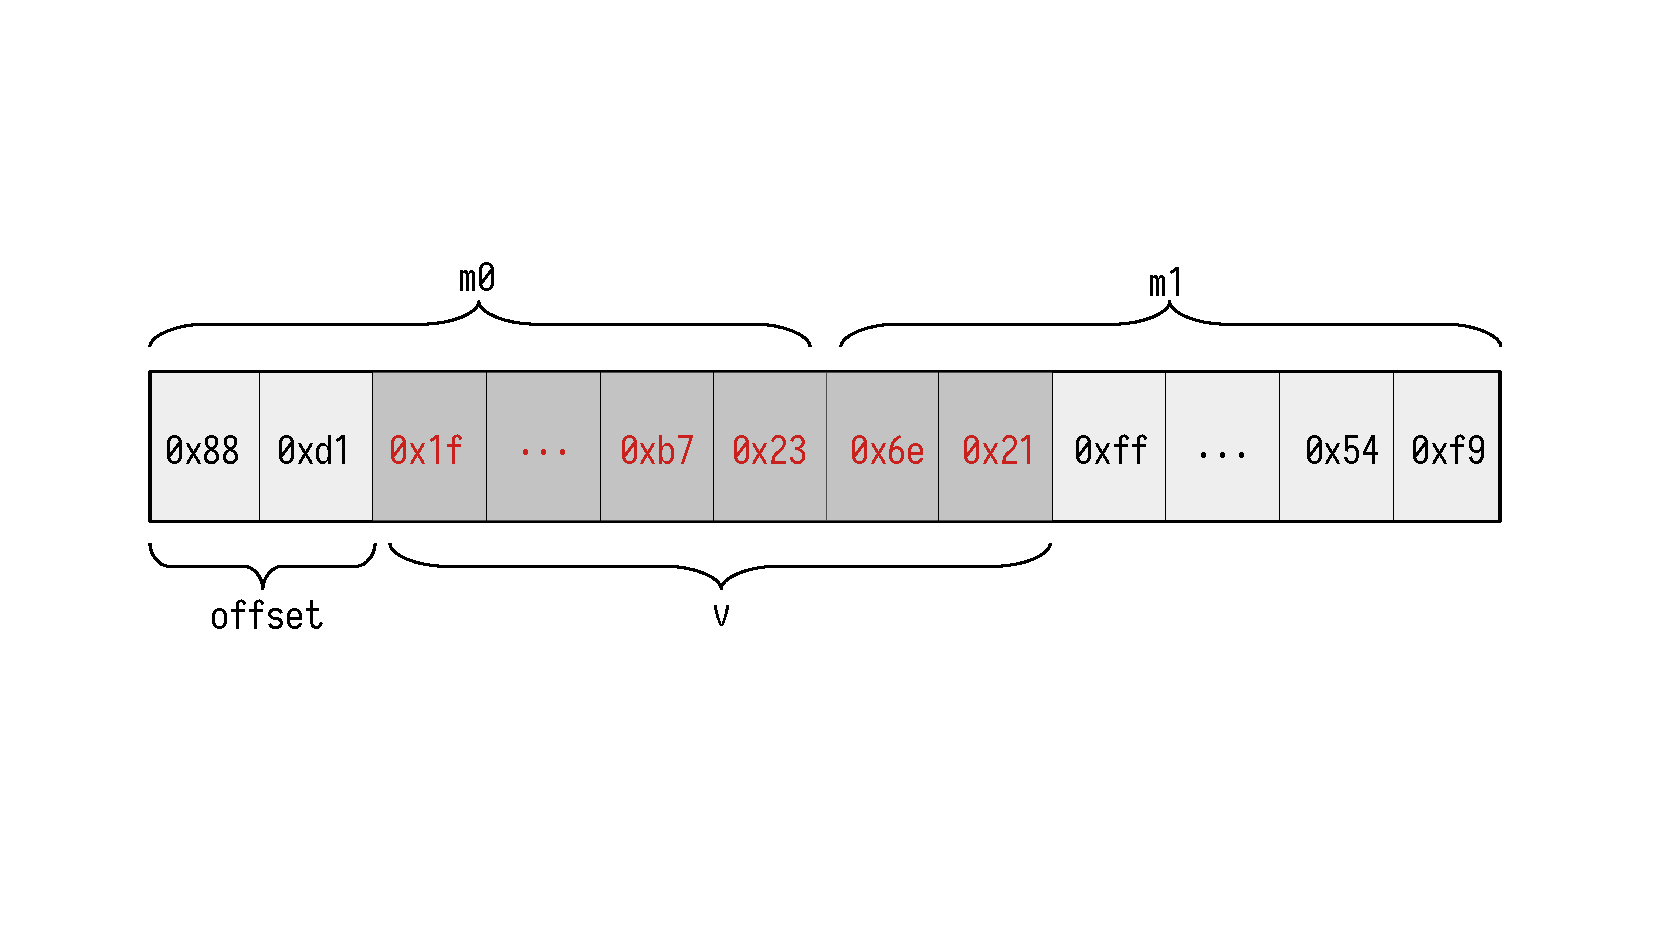
\includegraphics[width=1\columnwidth, trim=0 5cm 0 4cm, clip]{../figures/mload_ex}
    \caption{Schema of \MLOAD example.}
    \label{fig:mload-ex}
\end{figure}

Let us now introduce the flow at the time of validating a read. Suppose that we want to validate that if we perform an \MLOAD operation at the address $\mathtt{0x22}$, we get the previous value $\mathtt{0x1f\dotsb7236e21}$. At this point, the main state machine will perform several operations. First of all, it will have to query for the values \mF and \mS. Henceforth, it must call the \textbf{Memory SM} in order to validate the previous queries. 

Observe that it is easy to extract the memory positions to query from the address $\mathtt{0x22}$. In fact, if $a$ is the memory position of the \MLOAD operation, then \mF is always stored at the memory position $\lfloor \frac{a}{32} \rfloor$ and \mS is stored at the memory position $\lfloor \frac{a}{32} \rfloor + 1$. In our example, $a = \mathtt{0x22} = 34$. Hence, \mF is stored at the position $\lfloor \frac{32}{34} \rfloor = \mathtt{0x01}$ and \mS is stored at the position $\lfloor \frac{32}{34} \rfloor + 1= \mathtt{0x02}$. 

Secondly, we should extract the correct \offset. The \offset represents an index between $0$ and $31$ indicating the number of bytes we should offset from the starting of \mF to correctly place \val in the block. In our case, the \offset is $2$. Similarly as before, it is easy to obtain the offset from $a$. In fact, the it is equal to $a \mod{32}$. Now, the \textbf{Main SM} will check against the Memory Align State Machine that \val is a correct read given the affected words \mF and \mS and the \offset. That is, we should check that the value $\val$ can be correctly split into \mF and \mS using the provided \offset. 


Similarly, \MSTORE instruction requires, in general, writing bytes in two words.
The idea is very similar, but we are provided with a value \val that we want to write into a specific location of the memory. We will denote by \wF and \wS the words that arise from \mF and \mS after the corresponding write. 

Following our previous example, suppose that we want to write 
\[
\val = \mathtt{0xe201e6\dots662b}
\] 
in the address \texttt{0x22} of the byte-addressed Ethereum memory. We are using the same \mF and \mS (and since we are writting into the same address as before) and they will transition into  (see Figure \ref{fig:mstore-ex}):
\[
\wF = \mathtt{0x88d1}\color{-red!75}\mathtt{e201e6\dots}\color{black},\quad \wS =  \mathtt{0x}\color{-red!75} \mathtt{662b}\color{black} \mathtt{ff\dots54f9}.
\]

\begin{figure}[h!]
    \centering
    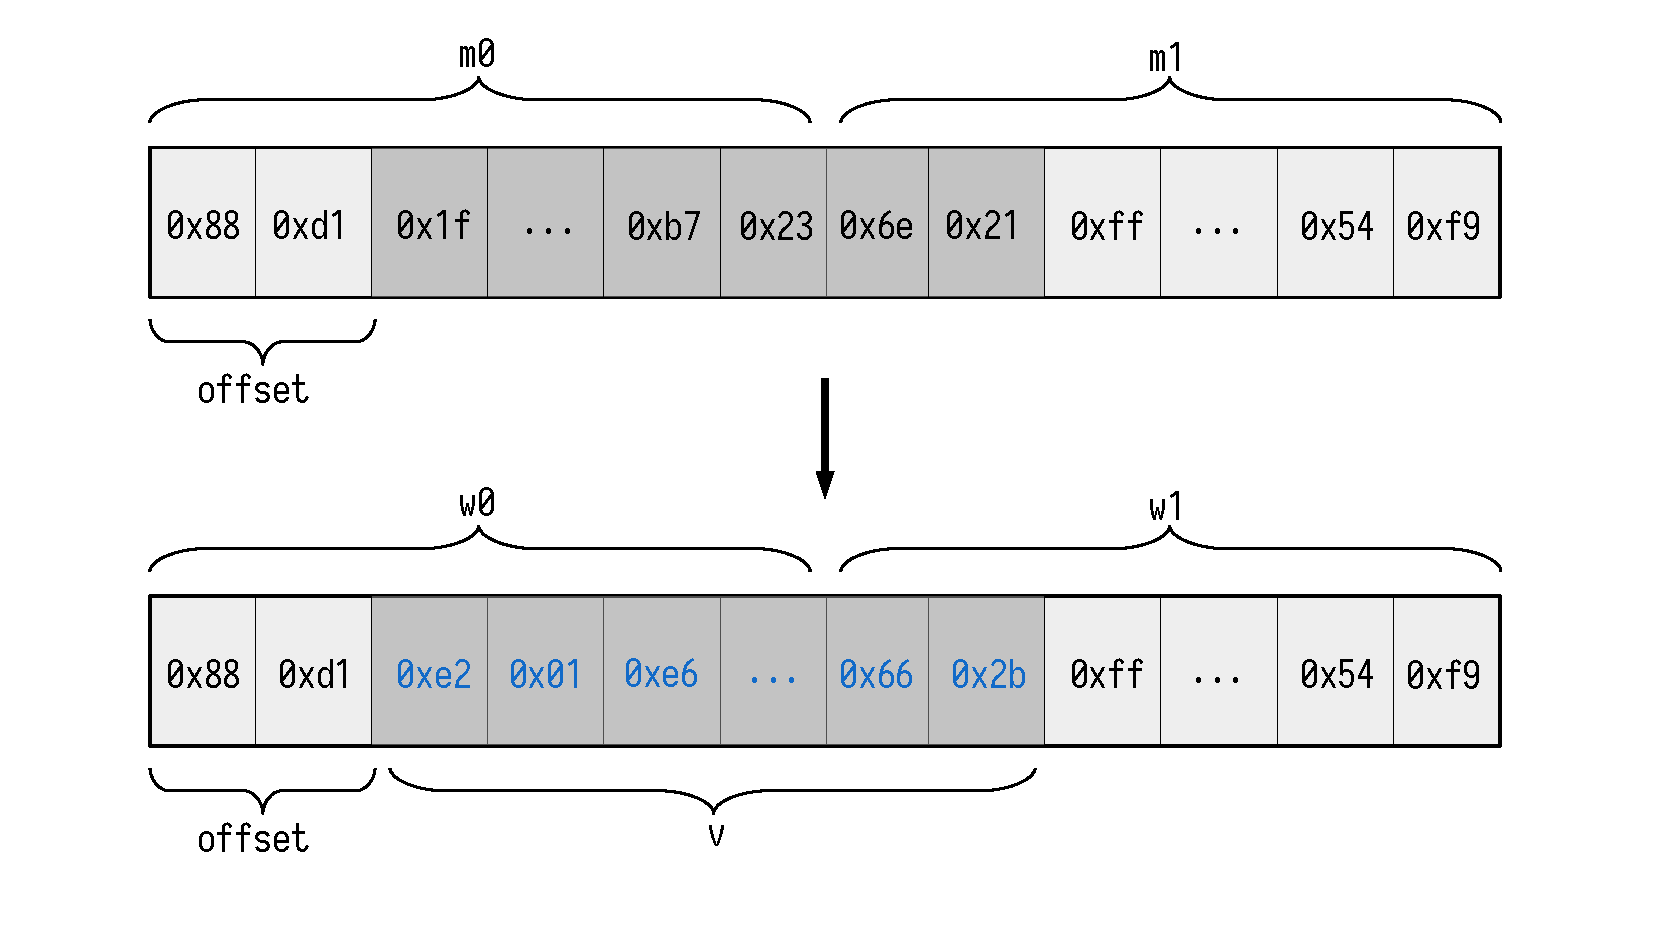
\includegraphics[width=1\columnwidth]{../figures/mstore_ex}
    \caption{Schema of \MSTORE example.}
    \label{fig:mstore-ex}
\end{figure}

Just as before, the main state machine will need to perform several operations. We will be given an address \addr, an offset value \offset and a value to be wrote \val. Identically as before, the \textbf{Main SM} will be in charge of reading the zkEVM memory to find \mF and \mS from the given address and offset. Of course, the validity of this query should be performed with a specific Plookup into the \textbf{Memory SM}, just as before. 

Now, the \textbf{Main SM} can compute \wF and \wS from all the previous values in a uniquely way. The way of validating that we are providing the correct \wF and \wS is to perform a Plookup into the \textbf{Memory Align SM}. That is, we will check that the provided values \wF and \wS are correctly constructed from the provided \val, \mF, \mS and \offset values. 


Finally, the last opcode \MSTOREE works similarly, \textit{but it only affects one word} \mF. Moreover, we can only write one byte and hence, only the less significant byte of \val will be considered into the write. Observe that, in this opcode, \mS and \wS are unconstrained.




\subsection{Storage SM}


The \textbf{Storage SM} is  in charge of validate operations over the key-value storage structure present in the EVM. The \textbf{Storage SM} is an essential building block for designing a more generic virtual machine that can check the correctness of state transitions resulting from executing smart contract transactions. The keys are expressed with 4 elements of $\FF_p$, while the values are expressed using 8 elements in $\FF_p$, where each of these eight elements have 0's at their most 32 significant bits.


The operations over the \textbf{Storage SM} are the typical Create, Read, Update and Delete (CRUD). A specific behavior of the \textbf{Storage SM} is that, in read operations, it returns zero if a key is not found. The structure used to build the key-value storage that can be proven with zero knowledge is a specific variant 
of a Merkle Patricia Tree (MPT).

In general, a Merkle tree is a data structure where every \emph{leaf} of the tree contains the cryptographic hash of a value and every \emph{non leaf}, which we also denote as \emph{branch}, contains the concatenated hashes of its children. Merkle trees allow to link a set of values to a unique hash called the \emph{root} of the tree and the efficient and secure verification of containment of large sets of key-values. In our case, we will use the key to unequivocally determine the position of the leaf in the Merkle tree. Furthermore, we are going to use the previously explained Poseidon hash function because it is a function that can be verified with zero-knowledge primitives in a more friendly way than other standard hash functions like KECCAK. Moreover, two different instances of Poseidon hash function (achieved modifying the initial value for the capacity) should be used for hashing leafs and branches to prevent possible attacks. 

The mechanics of the particular MPT proposed and its operations are described in detail later but essentially, proving operations over this hash structure involves to types of checks:

\begin{itemize}
    
    \item For read operations, we need to show that the value of a related key is included at the tree at the correct position.
    
    \item For write operations, we have to prove that modifications lead to the appropriate new root.
    
\end{itemize}




\subsection{Counters}

Counters are a mechanism to control that the total number of steps do not exceed the maximum polynomial size. The purpose of counters is to limit the number of steps that can be taken during the processing of a transaction, in order to ensure that the computation terminates within a certain time bound, defined by the polynomial size, currently stored in a constant

\begin{zkasm}
    CONST %TOTAL_STEPS = 2**23
\end{zkasm}
to prevent the cryptographic proof system from failing due to a denial-of-service attack. Additionally, it is important to consider that there is a fixed minimum number of steps required to complete the processing of a transaction:

\begin{zkasm}
    CONST %MIN_STEPS_FINISH_BATCH = 200 
\end{zkasm}

As a result, the total number of steps is determined by the following variable:

\begin{zkasm}
    CONST %MAX_CNT_STEPS = %TOTAL_STEPS - %MIN_STEPS_FINISH_BATCH
\end{zkasm}

Since there are operations that are more often used than others, it is a really good practice to limit the steps for each of the state machines individually. The values assigned to these counters are typically derived through a combination of design considerations and empirical testing. Design considerations may include factors such as the expected input rate or the maximum number of cycles the system can handle before failure. Empirical testing may involve running simulations or testing the system in a real-world environment to determine appropriate counter values.

\begin{zkasm}
    CONST %MAX_CNT_ARITH = %TOTAL_STEPS / 32
    CONST %MAX_CNT_BINARY = %TOTAL_STEPS / 16
    CONST %MAX_CNT_MEM_ALIGN = %TOTAL_STEPS / 32
    CONST %MAX_CNT_KECCAK_F = (%TOTAL_STEPS / 155286) * 44
    CONST %MAX_CNT_PADDING_PG = (%TOTAL_STEPS / 56)
    CONST %MAX_CNT_POSEIDON_G = (%TOTAL_STEPS / 30)
\end{zkasm}
